\documentclass[a4paper]{scrreprt}

\usepackage[german]{babel}
\usepackage[utf8]{inputenc}
\usepackage[T1]{fontenc}
\usepackage{ae}
\usepackage[bookmarks,bookmarksnumbered]{hyperref}
\usepackage{graphicx}
\usepackage[toc]{glossaries}
\usepackage{tocbasic}
\graphicspath{ {images/} }
\setcounter{secnumdepth}{5}
\makeglossaries

\begin{document}
	\newglossaryentry{Android-App}
	{name=Android-App, description={Anwendungssoftware für Mobilgeräte mit Android als Betriebssystem}}
	
    \begin{flushright}
        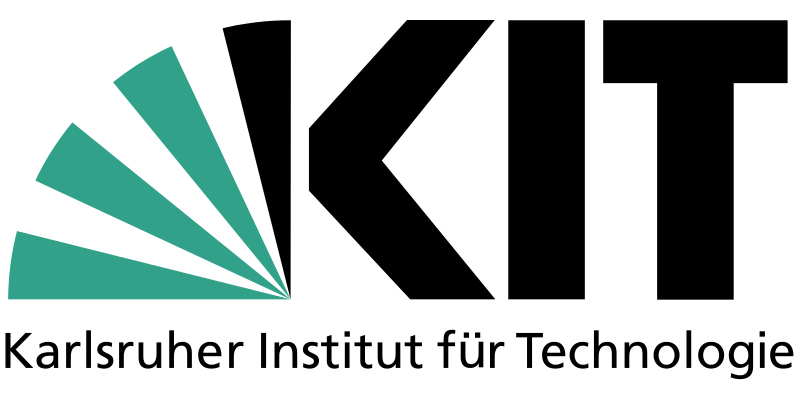
\includegraphics[scale = 0.2]{kit-logo.png}\\[0.5cm]
    \end{flushright}
    \vspace*{2cm}

    \begin{center} 
    		\large Praxis der Softwareentwicklung
        \vspace*{1.5cm}

        \textbf{\huge [Thema]}
        \vspace*{1cm}

        \textbf{\Large Pflichtenheft}
        \vspace*{2cm}

        [Name]
        \vspace*{1cm}

        [Datum]
        \vspace*{2.5cm}

        [Betreuung]\\[0.5cm]
        [Forschungsgruppe]\\[0.5cm]

        Karlsruher Institut für Technologie
    \end{center}
    \thispagestyle{empty}

    \tableofcontents

    \chapter{Zielbestimmung}
        \section{Musskriterien}

        \section{Wunschkriterien}

        \section{Abgrenzungskriterien}

    \chapter{Produkteinsatz}

        \section{Anwendungsbereiche}

        \section{Zielgruppen}

        \section{Betriebsbedingungen}

    \chapter{Produktumgebung}
        \section{Software}

        \section{Hardware}

    \chapter{Funktionale Anforderungen}

    \chapter{Produktdaten}

    \chapter{Nichtfunktionale Anforderungen}	

    \chapter{Testfälle}

    \chapter{Systemmodelle}
        \section{Szenarien}

        \newpage
        \section{Anwendungsfalldiagramm}

        \newpage
        \section{Benutzerschnittstelle}

    \glsaddall
    \printglossary

    \listoffigures

\end{document}